% Created by tikzDevice version 0.10.1 on 2018-07-11 20:12:48
% !TEX encoding = UTF-8 Unicode
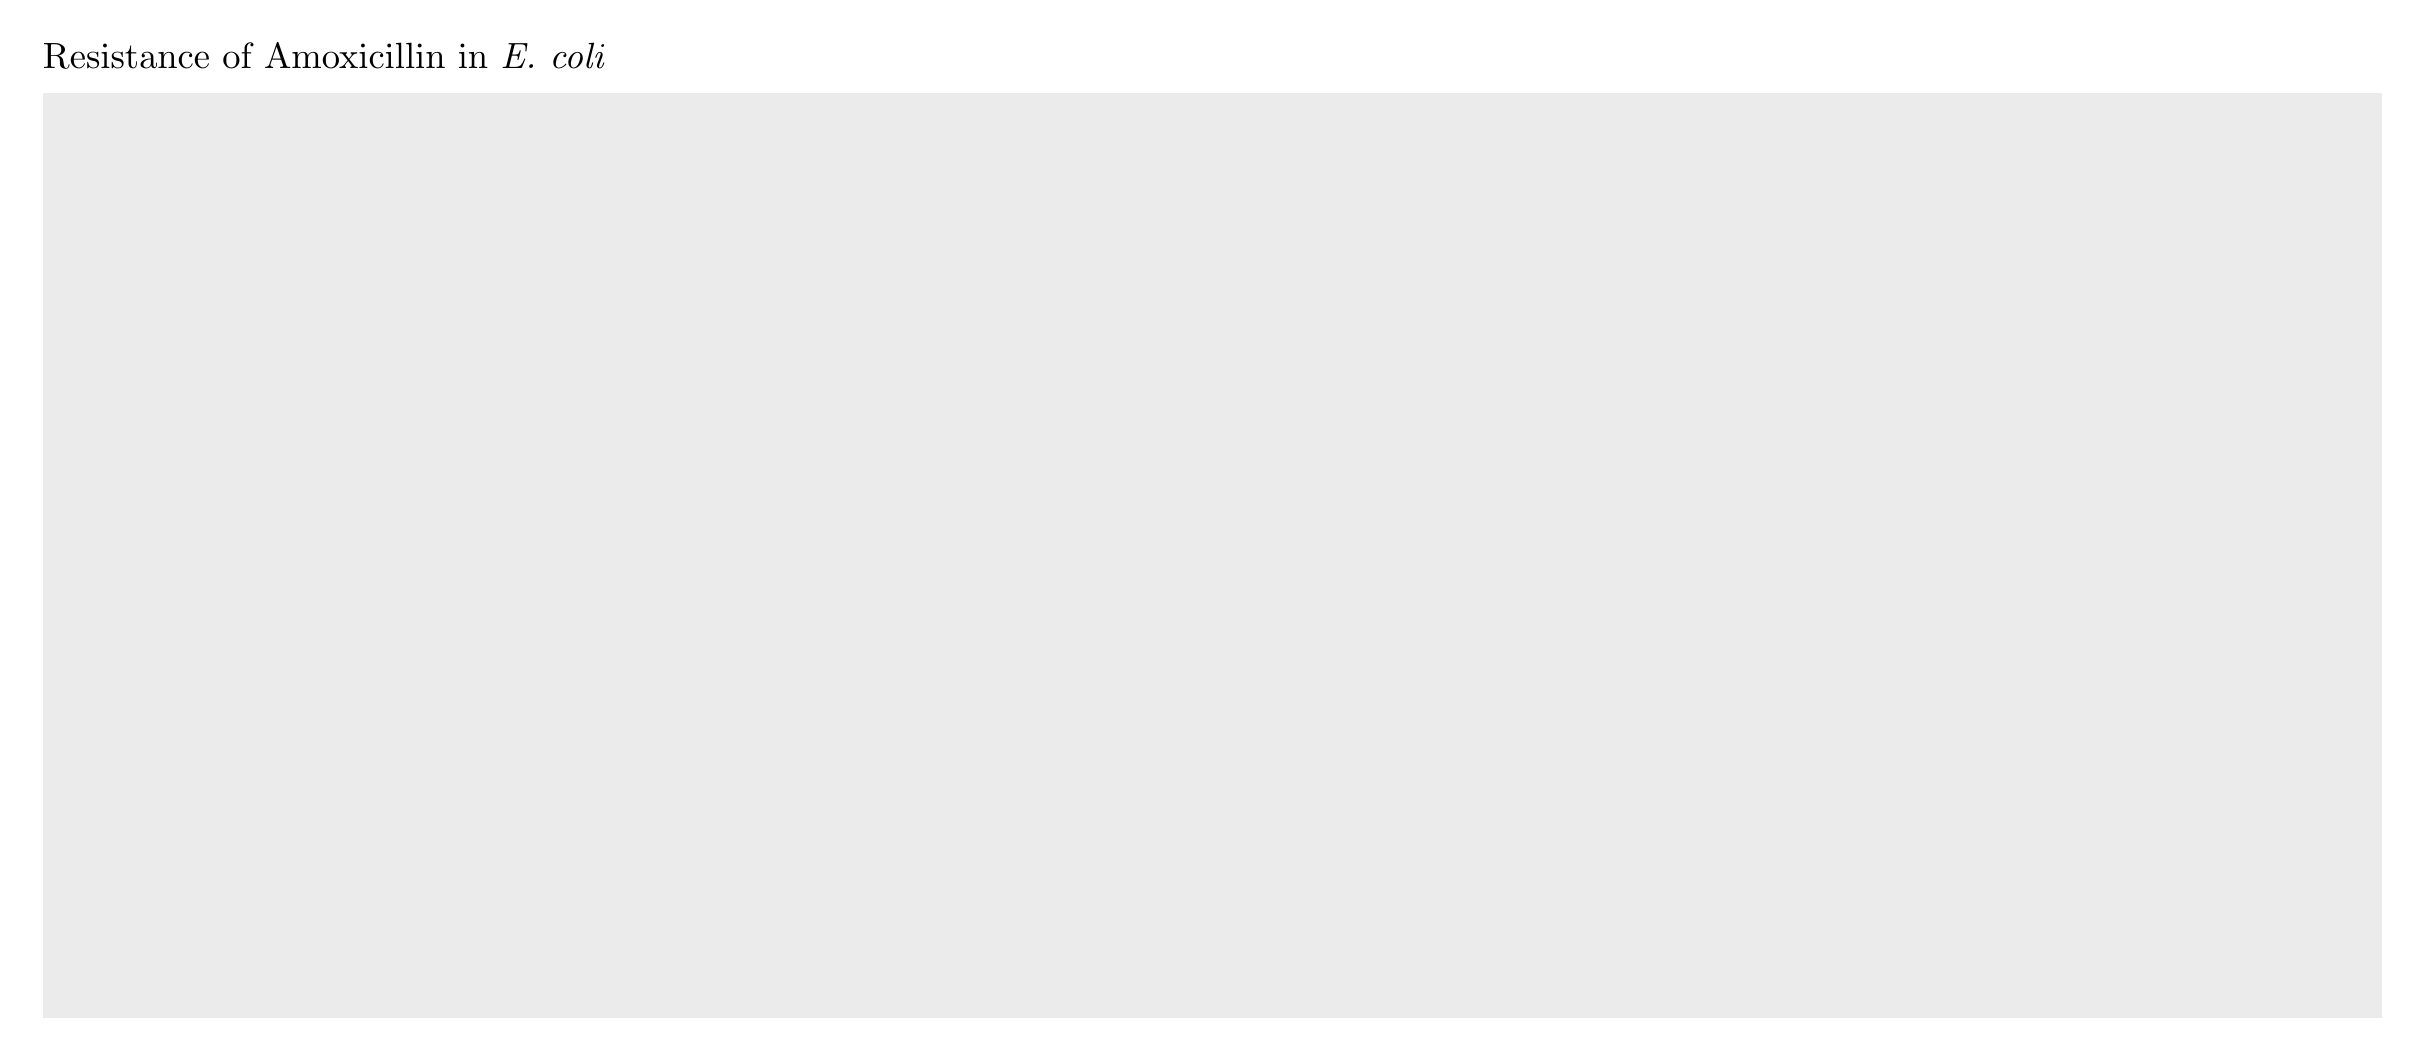
\begin{tikzpicture}[x=1pt,y=1pt]
\definecolor{fillColor}{RGB}{255,255,255}
\path[use as bounding box,fill=fillColor,fill opacity=0.00] (0,0) rectangle (856.20,363.36);
\begin{scope}
\path[clip] (  0.00,  0.00) rectangle (856.20,363.36);
\definecolor{drawColor}{RGB}{255,255,255}
\definecolor{fillColor}{RGB}{255,255,255}

\path[draw=drawColor,line width= 0.6pt,line join=round,line cap=round,fill=fillColor] (  0.00,  0.00) rectangle (856.20,363.36);
\end{scope}
\begin{scope}
\path[clip] (  5.50,  5.50) rectangle (850.70,339.67);
\definecolor{fillColor}{gray}{0.92}

\path[fill=fillColor] (  5.50,  5.50) rectangle (850.70,339.67);
\end{scope}
\begin{scope}
\path[clip] (  0.00,  0.00) rectangle (856.20,363.36);
\definecolor{drawColor}{RGB}{0,0,0}

\node[text=drawColor,anchor=base west,inner sep=0pt, outer sep=0pt, scale=  1.32] at (  5.50,348.77) {Resistance of Amoxicillin in \emph{E. coli}};
\end{scope}
\end{tikzpicture}
